\documentclass[serif,xcolor=pdftex,dvipsnames,table,hyperref={bookmarks=false,breaklinks}]{beamer}

%%%%%%%%%%%%%%%%
% Change the macros below to configure the title slides
% for your course.
\newcommand{\coursename}{COMPSCI 589}
\newcommand{\instructor}{Benjamin M. Marlin}
\newcommand{\university}{University of Massachusetts Amherst}
\newcommand{\department}{College of Information and Computer Sciences}
%%%%%%%%%%%%%%%%


\newcommand{\settitlecard}[2]{
  \title[\coursename  Lecture #1] 
    {\coursename \\ Lecture #1: #2}
     \author[\instructor]{\instructor}
     \institute[\university]{
     \department\\
     \university
   }
\date{}
}

\newcommand{\maketitlepage}{
  \begin{frame}
  \titlepage
  \center{
    %If you use the slides unmodified, retain the attribution below
    \tiny{Slides by Benjamin M. Marlin (marlin@cs.umass.edu). \\
    \vspace{-1em}Created with support from National Science Foundation Award\# IIS-1350522. 
    %If you modify the slides, please retain the alternate attribution below
    %\tiny{Based on slides by Benjamin M. Marlin (marlin@cs.umass.edu). \\    
    %\vspace{-1em}Created with support from National Science Foundation Award\# IIS-1350522. 
    }                                              
  }  
  \end{frame}
}

\AtBeginSection[]
{
  \begin{frame}<beamer>{Outline}
    \tableofcontents[currentsection,subsectionstyle=hide]
  \end{frame}
}


\newcommand{\cut}[1]{}

\newcommand{\iconbox}[4]{
  \only<#1-#2>{
    \begin{columns}[T]
      \column{0.5in}
           \includegraphics[width=0.5in]{#3}
       \column{3.7in}
            #4
    \end{columns}
    \medskip
    \medskip
    \medskip
  }
}

\mode<presentation>{
  \usepackage{../beamertheme589theme}
  \setbeamercovered{invisible}
}

\mode<handout>{
  \usepackage{../beamertheme589theme}
  \setbeamercovered{transparent}
}


\usepackage[english]{babel}
\usepackage[latin1]{inputenc}
\usepackage{times}
\usepackage[T1]{fontenc}
\usepackage{amsmath}
\usepackage{amssymb}
\usepackage[noend]{algorithmic}
\usepackage{algorithm}
\usepackage{listings}

\renewcommand\mathfamilydefault{\rmdefault}

\newcommand{\setA}{\mathcal{A}}
\newcommand{\setB}{\mathcal{B}}
\newcommand{\setS}{\mathcal{S}}
\newcommand{\setV}{\mathcal{V}}
\DeclareMathOperator*{\union}{\bigcup}
\DeclareMathOperator*{\intersection}{\bigcap}
\DeclareMathOperator*{\Val}{Val}
\newcommand{\mbf}[1]{{\mathbf{#1}}}
\DeclareMathOperator*{\argmax}{arg\,max}
\DeclareMathOperator*{\argmin}{arg\,min}
\DeclareMathOperator*{\sign}{sign}
\newcommand{\deriv}[2]{\frac{\partial{#1}}{\partial{#2}}}


\settitlecard{20}{Sparse Coding, NMF and ICA}

\begin{document}

\maketitlepage


\section{Review}
\subsection{Foo}

\begin{frame}[t]{Linear Dimensionality Reduction}
 
\begin{itemize}
\item The learning problem for linear dimensionality reduction is to estimate
values for both $\mbf{Z}$ and $\mbf{B}$ given only the noisy observations 
$\mbf{X}$.

\item One possible learning criteria is to minimize the sum of squared 
errors when reconstructing $\mbf{X}$ from $\mbf{Z}$ and $\mbf{B}$. This leads 
to:

{\Large
$$\argmin_{\mbf{Z},\mbf{B}} ||\mbf{X} - \mbf{Z}\mbf{B} ||_F$$
}

where $||\mbf{A}||_F$ is the Frobenius norm of matrix  $\mbf{A}$ (the sum of 
the squares of all matrix entries). 

\end{itemize} 
\end{frame}

\begin{frame}[t]{PCA and SVD}

\begin{itemize}
\item PCA on $\mbf{X}^T\mbf{X}$ and SVD on 
$\mbf{X}$ identify exactly the same linear sub-space and result in exactly the 
same projection of the data into that linear sub-space.

\item As a result, generic linear dimensionality reduction 
simultaneously minimizes the Frobenius norm of the reconstruction error of 
$\mbf{X}$ and maximizes the retained variance in the learned sub-space.

\item SVD and PCA provide the same refinement of generic linear 
dimensionality reduction: an orthogonal basis for exactly the same optimal 
linear subspace. 

\item To extend PCA and SVD to the non-linear case, we can use basis expansions 
or kernels (next class).

\end{itemize} 
\end{frame}


\begin{frame}[t]{Limitations}

\begin{itemize}
\item PCA and SVD constrain the basis elements to be orthonormal. 

\pause\item In some cases we may want to extract representations where the 
basis elements and factor loadings are non-negative, representations where the 
factor loadings are maximally independent, or representations where the 
factor loadings are sparse.

\pause\item The reason is that these constraints may better 
model the process that generates the data. These constraints may also help 
with recognition tasks.

\end{itemize} 
\end{frame}

\section{Sparse Coding}
\subsection{Foo}

\begin{frame}[t]{Sparse Coding}

\begin{itemize}
\item Sparse coding is an extension of linear dimensionality reduction where 
the factor loadings are constrained to be sparse.

\pause\item This model is closely related to the Lasso ($\ell_1$ 
regularized linear regression).
 
\pause\item This gives rise to the following optimization problem:

{\Large
\begin{align*}
&\min_{\mbf{Z},\mbf{B}} ||\mbf{X} - \mbf{Z}\mbf{B} ||_F - 
\lambda||\mbf{Z}||_1 \\
&\mbox{such that } ||B_k||_2=1 \mbox{ for all } k
\end{align*}
}
 
where $||\mbf{A}||_1$ is the sum of the absolute values of the elements in 
$\mbf{A}$ and $||\mbf{A}||_F$ is the sum of the squares of the elements in 
$\mbf{A}$. 
 
\end{itemize} 
\end{frame}

\begin{frame}[t]{Motivation}

\begin{itemize}
\item By the early 2000's several theoretical, computational, and experimental 
studies suggested that neurons encode sensory information using a small
number of active neurons at any given point in time, a strategy that was named
sparse coding in the computational neuroscience literature.

\pause\item Olshausen and Field (2004) argued that sparse coding makes 
the structure in natural signals more apparent, represents complex data in a 
way that is easier to read out in later stages of processing, and saves energy.

\pause\item As $\lambda$ increases, the representation becomes sparser, 
typically using a small number of the $K$ available basis vectors to encode 
each signal. By comparison, the PCA representation of a natural signal normally 
puts non-zero weight on all basis elements.

\end{itemize}
\end{frame}

\begin{frame}[t]{Example: Image Patches}
\center
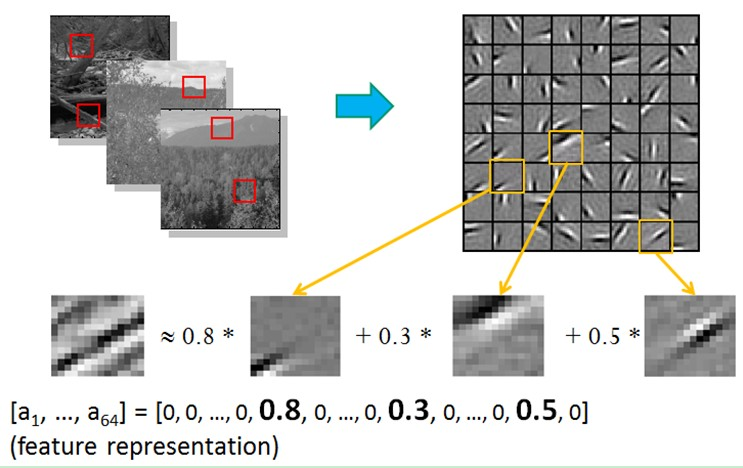
\includegraphics[width=4.5in]{../Figures/sparse_coding_images.jpg}
\end{frame}

\begin{frame}[t]{Example: Time Series}
\center
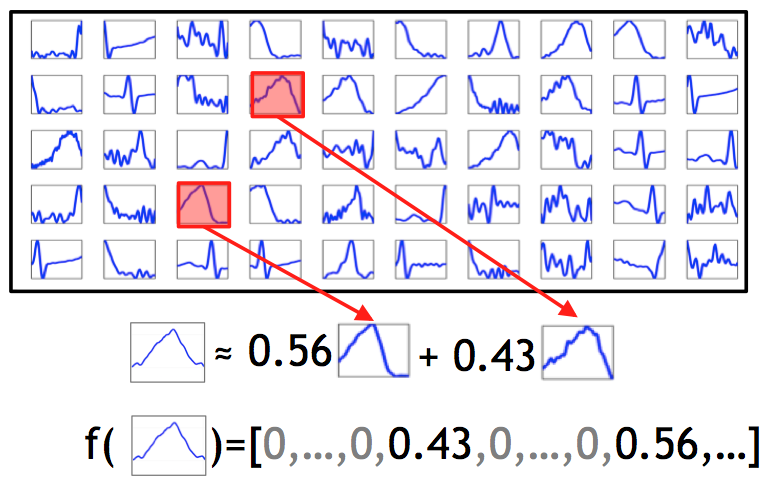
\includegraphics[width=4in]{../Figures/spase_coding_time_series.png}
\end{frame}

\section{NMF}
\subsection{Foo}

\begin{frame}[t]{Non-Negative Matrix Factorization}

\begin{itemize}
\item NMF is an extension of linear dimensionality reduction where 
the factor loadings and the basis elements are constrained to be positive.
 
\pause\item This gives rise to the following optimization problem:

{\Large
\begin{align*}
&\min_{\mbf{Z},\mbf{B}} ||\mbf{X} - \mbf{Z}\mbf{B} ||_F\\
&\mbox{such that } \mbf{B}\geq 0, \mbf{Z}\geq 0
\end{align*}
}
 
\end{itemize} 
\end{frame}

\begin{frame}[t]{Motivation}

\begin{itemize}
\item Data including natural images, gene expressions, and word count 
representations of text are naturally non-negative.

\pause\item In many cases, complex non-negative data arise from a 
non-negative composition of simpler non-negative parts.

\pause\item This is exactly the intuition that non-negative matrix 
factorization is designed to capture.


\end{itemize}
\end{frame}

\begin{frame}[t]{Example: Learning Face Parts}
\center
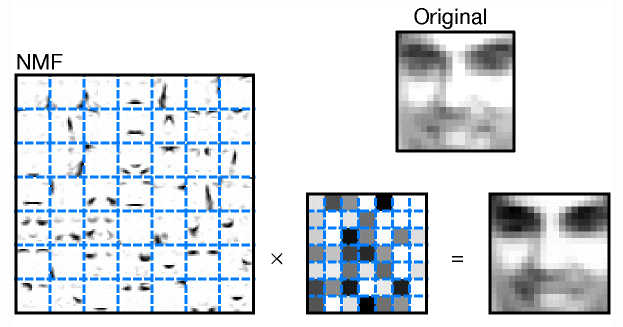
\includegraphics[width=4.5in]{../Figures/nmf.png}
\end{frame}

\section{ICA}
\subsection{Foo}

\begin{frame}[t]{Independent Components Analysis}

\begin{itemize}
\item ICA is an extension of linear dimensionality reduction where 
the random variables that represent the factor loadings are constrained to be 
problematically independent of each other.  
 
\pause\item This gives rise to the following optimization problem:

{\Large
\begin{align*}
&\min_{\mbf{Z},\mbf{B}} ||\mbf{X} - \mbf{Z}\mbf{B} ||_F\\
&\mbox{such that } Z_i \bot Z_j \mbox{ for all } 1<i<j<k
\end{align*}
}

\pause\item In practice, a surrogate criterion must be used in place of 
independence and a number of different functions have been explored in the 
literature.  

\end{itemize} 
\end{frame}

\begin{frame}[t]{Motivation}

\begin{itemize}
\item Linear mixing of independent sources is exactly what occurs when you
listen to multiple audio sources at the same time.

\pause\item Humans are somehow able to automatically de-mix multiple sources of 
audio (multiple people speaking) into distinct source channels very accurately.

\pause\item ICA was designed to solve exactly this problem (called blind source 
separation) and can do so very reliably when the number of observed linearly 
mixed channels is equal to the number of sources.

\pause\item The method has also been applied to images and many other types of 
data.

\end{itemize}
\end{frame}

\begin{frame}[t]{Example: Blind Source Separation}
\center
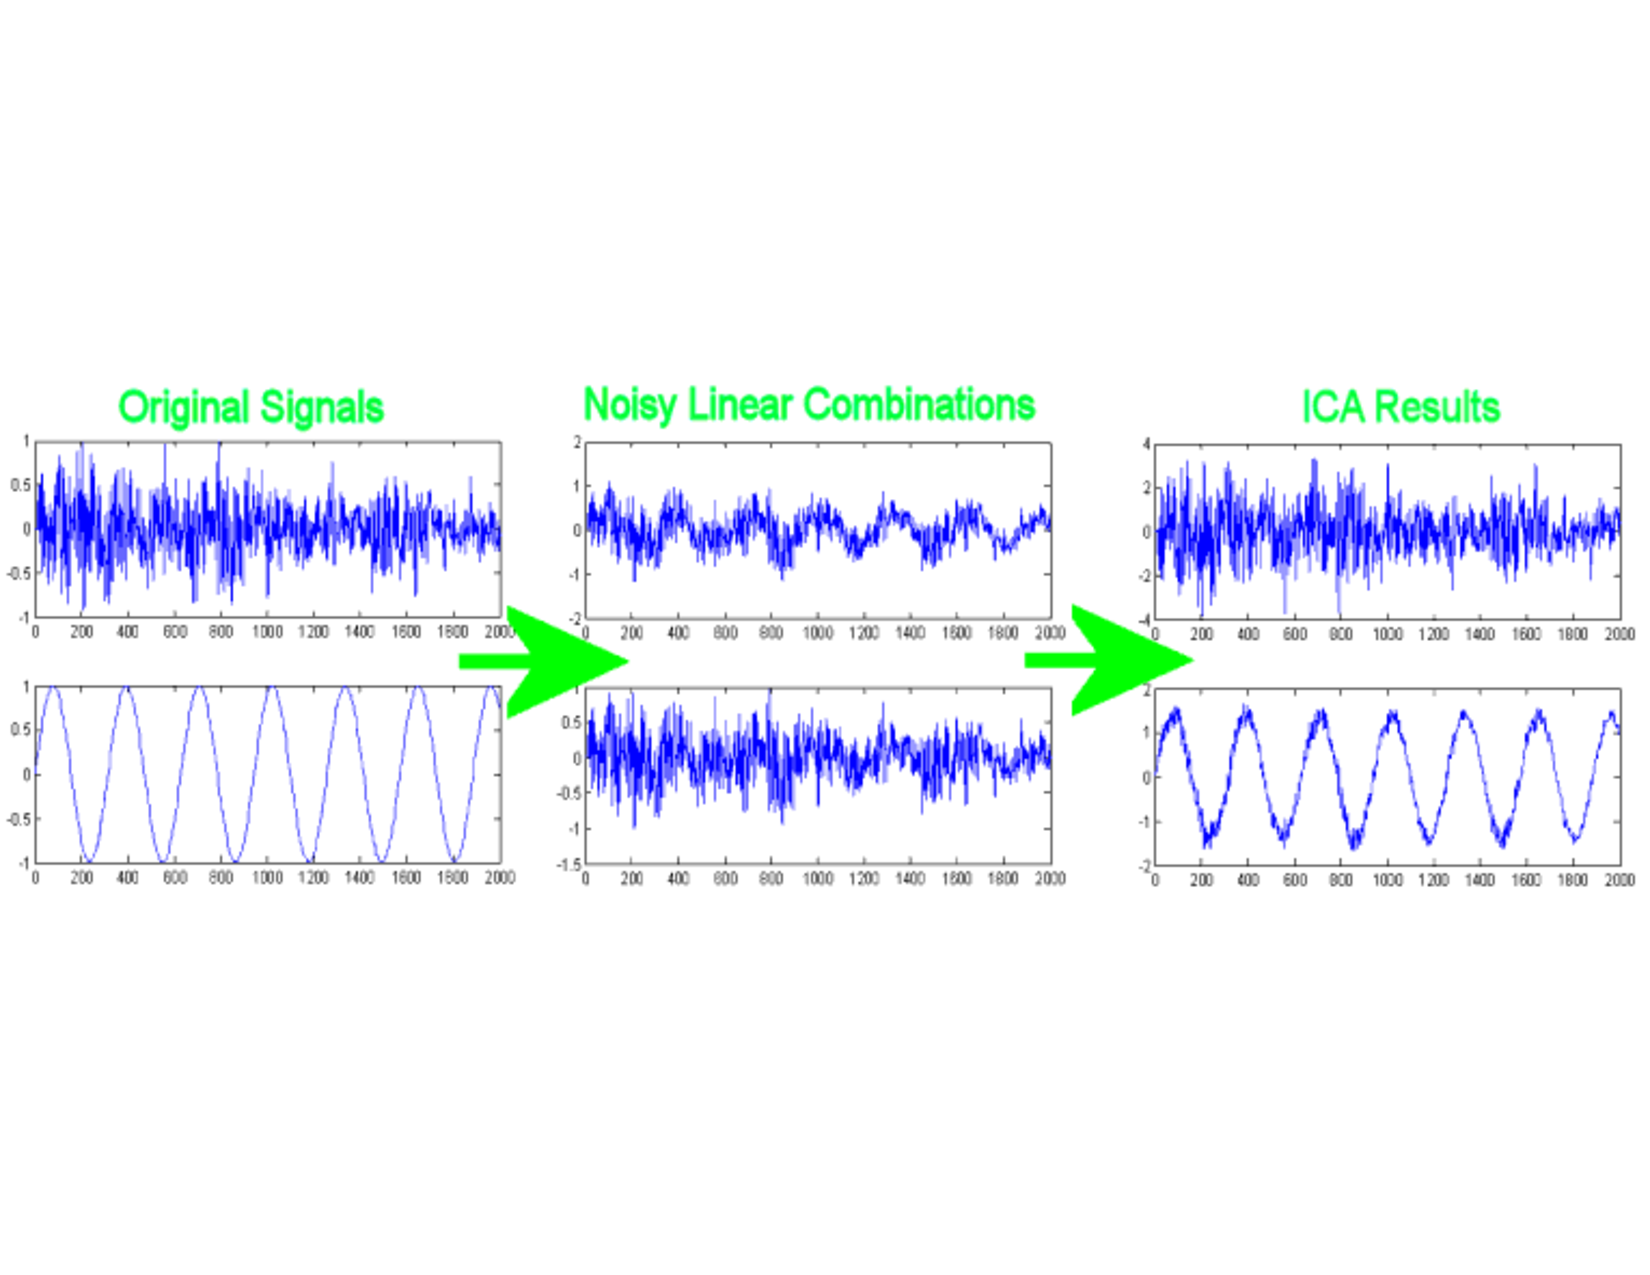
\includegraphics[width=4.5in]{../Figures/ica_signals.pdf}
\end{frame}


\begin{frame}[t]{Example: Independent Components of Natural Images}
\center
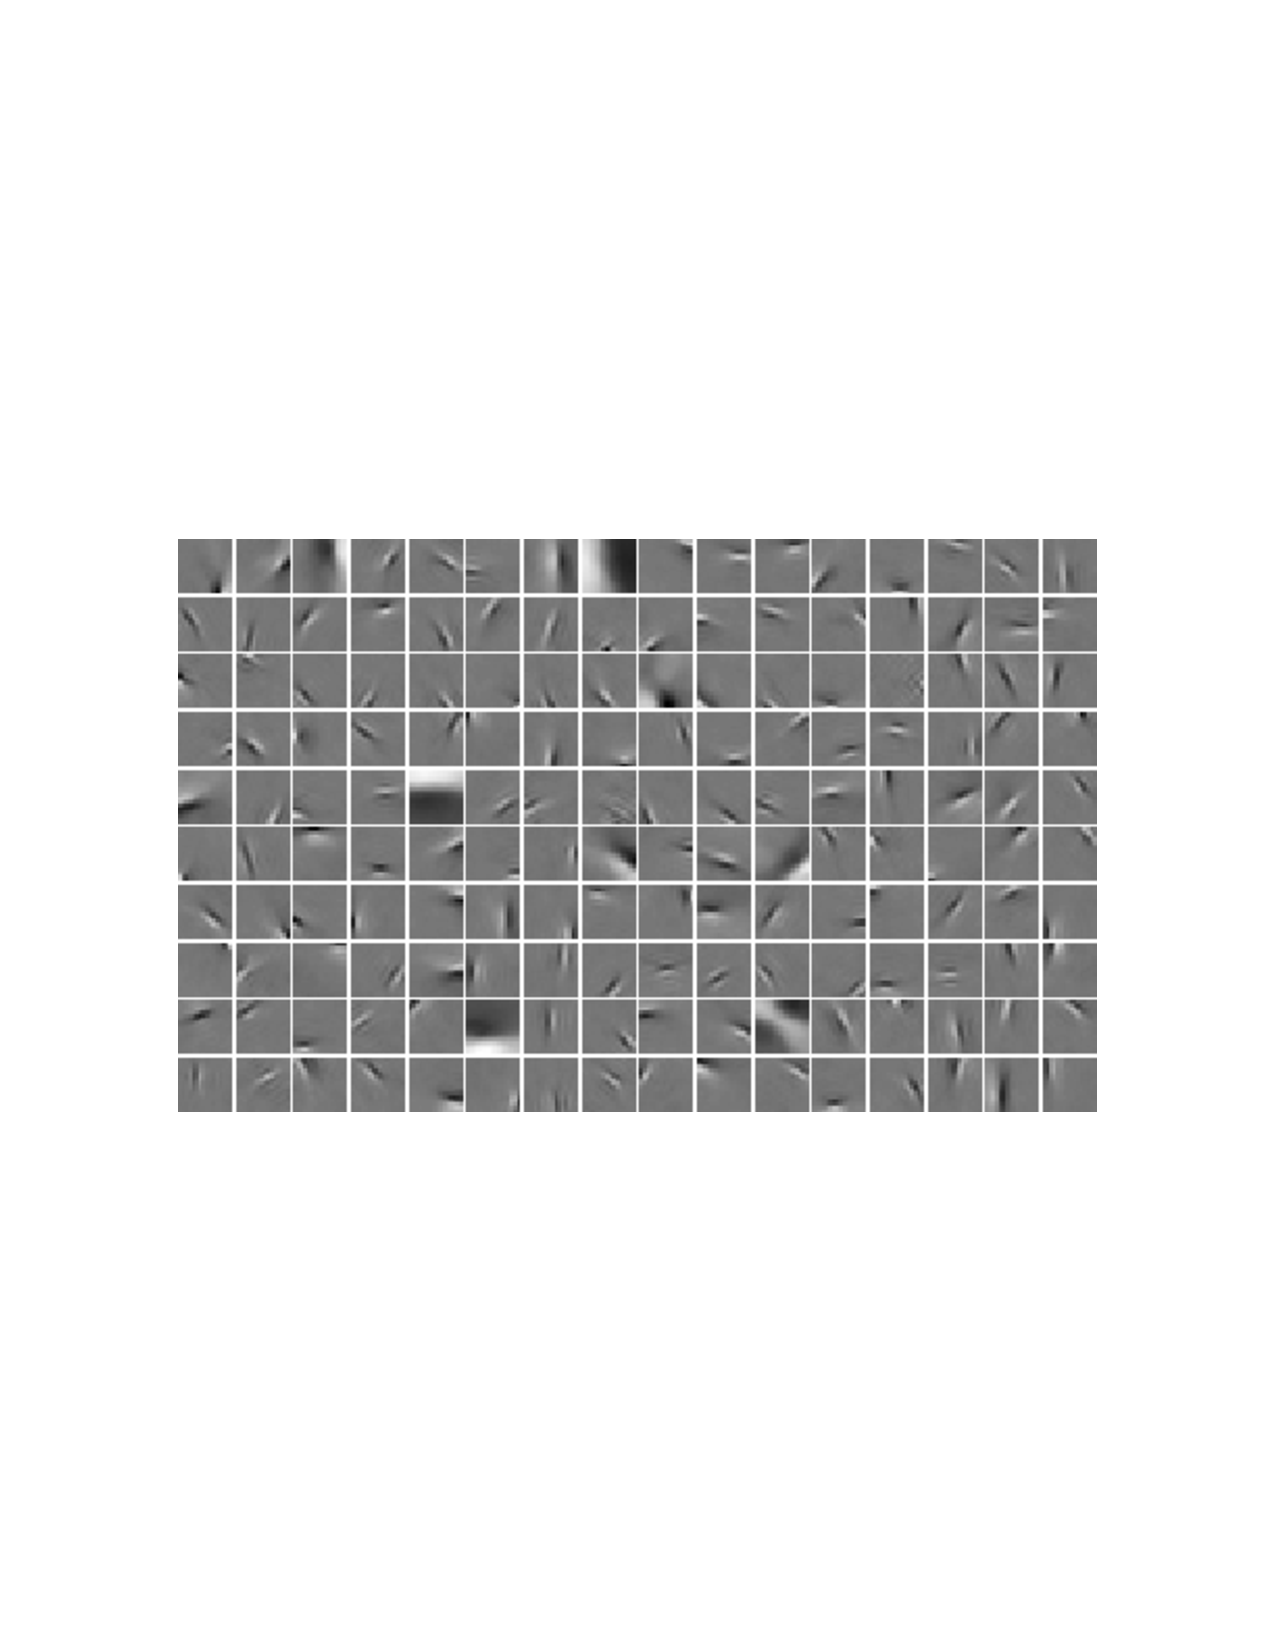
\includegraphics[width=4.5in]{../Figures/ica_images.pdf}
\end{frame}






\end{document}
